%% report_template.tex
%% V1.0
%% 2012-03-16
%% by Jesper Pedersen Notander
%% See:
%% http://www.cs.lth.se/jesper_pedersen_notander
%% for current contact information.
%%
%% This is a template file contaning instructions and a skeleton outline
%% for the final report in the course ETSA05: Software Engineering
%% Process - Soft Issues, given by the Department of Computer Science at
%% Lund University, Sweden.
%%
%% This template requires IEEEtran.cls, written by Michael Shell, version
%% 1.7 or later.
%%
%% Support sites:
%% http://www.cs.lth.se/etsa05/
%% http://www.ieee.org/

%%*************************************************************************
%% Legal Notice:
%% This code is offered as-is without any warranty either expressed or
%% implied; without even the implied warranty of MERCHANTABILITY or
%% FITNESS FOR A PARTICULAR PURPOSE!
%%
%% User assumes all risk.
%%
%% In no event shall Lund University or any contributor to this code be
%% liable for any damages or losses, including, but not limited to,
%% incidental, consequential, or any other damages, resulting from the use
%% or misuse of any information contained here.
%%
%% All comments are the opinions of their respective authors and are not
%% necessarily endorsed by Lund University.
%%
%% This work is distributed under the LaTeX Project Public License (LPPL)
%% ( http://www.latex-project.org/ ) version 1.3, and may be freely used,
%% distributed and modified. A copy of the LPPL, version 1.3, is included
%% in the base LaTeX documentation of all distributions of LaTeX released
%% 2003/12/01 or later.
%%
%% Retain all contribution notices and credits.
%% ** Modified files should be clearly indicated as such, including  **
%% ** renaming them and changing author support contact information. **
%%
%% File list of work: report_template.tex
%%*************************************************************************


\documentclass[conference]{IEEEtran}
\usepackage{graphicx}
% If IEEEtran.cls has not been installed into the LaTeX system files,
% manually specify the path to it like:
% \documentclass[conference]{../sty/IEEEtran}

\begin{document}

% TODO: examine the feasibility of this title before the submission
\title{On the Design of Software Processes and Software Process Improvement in
the Context of Lego Scrum Workshops}

% Leave as is to ensure anonymous grading.
\author{
\IEEEauthorblockN{ANONYMOUS AUTHOR}
\IEEEauthorblockA{Examination in DIT348 Software Development Methodologies\\
Department of Computer Science and Engineering\\
University of Gothenburg\\
Gothenburg, Sweden}}

\maketitle

\begin{abstract}
% This document is a template. The various components of your essay (title,
% headings, etc.) are already defined here. Please note that the headings
% must NOT change unless explicitly stated below. That is, you MUST use the
% predefined headings. Make sure to retain font sizes, line spacing, column
% width, and margins. Not following this template in either structure or
% layout will lead to a FAIL. Remember: the criteria for attaining the grades
% are defined in the course syllabus. To get a pass with distinction (5), you
% need to solve the bonus task (Section~\ref{sec:bonus_task}). Please replace
% this abstract with your own text, briefly state what this report is about,
% and summarize the key take-aways.

TODO
\end{abstract}

\section{Introduction}

% The introduction section should be used to introduce Software Processes and
% Software Process Improvement (SPI) in general and to introduce the purpose
% and context of this report.

A software process refers to the set of tools, methods, and practices used to
produce a software product \cite{Humphrey1989}.
With the increasing complexity of software systems, the need for a well-defined
software process has become more and more significant.
With that in mind, Basili and Rombach \cite{Basili1988} state that the software
engineering processes require \textbf{tailorability} because of the diversity
of the software products and the different environments in which they are
developed, hence the need for a software process improvement (hereafter SPI)
initiative.

This paper analyzes a designed software process and proposes an SPI initiative 
in the context of the Lego Scrum workshop that took place during the course.
Ultimately, ... % <TODO> (one sentence; a discussion topic or something like that). 

\section{Process Defined for the Scrum Workshop}
\label{sec:process}

% Describe the process you defined for the Scrum Lego Workshop. Explain whether
% you chose to apply Scrum, User Story Practice, and Incremental Delivery. Give
% reasons for why you did or did not use elements from these three practices.

The defined process is titled {\fontfamily{qhv}\selectfont AKAMMO} and primarily
utilizes concepts from Scrum and Incremental Delivery, and to a lesser extent,
User Story Practice. Scrum provides a flexible and adaptive approach to project
management, and encourages transparency in terms of the project's progress and
the issues encountered. Scrum, by definition, is meant to be applied in an
iterative manner, which is why a conjunction with Incremental Delivery becomes
a natural choice \cite{Srivastava2017}, \cite{Schwaber1997}.

Initially, the process assumes a set of user stories that are to be implemented
(and are prioritized by the Product Owner, hereafter PO). Afterwards, the team
members analyze the user stories and decide whether they require a further
elicitation of requirements (which is discussed with the PO) or whether they
can be implemented as they are.
Moreover, before each sprint, \textbf{sprint planning} takes place. It is an
activity that aims to split up the user stories into more granular requirements
that, once implemented, satisfy the acceptance criteria of a particular user
story, and, additionally, sprint planning is thought of as a way to delegate
requirements to the members of the team.

Subsequently, the requirements are assigned \textbf{story points} that
correspond to the difficulty of their implementation (i.e., the higher
the number, the more difficult the implementation) based on the Fibonacci
sequence. Strikingly, Tamrakar and Jørgensen \cite{Tamrakar2012} observe that
the Fibonacci scale (among other non-linear scales) eliminates the bias that is
introduced by any linear scale such that humans tend to be biased towards the
middle of the scale, and thereby non-linear scales yield more accurate results.

Furthermore, a \textbf{Kanban board} is to be used throughout the workshop to
categorize each user story into one of the following columns: (i) \textit{To
Do}, (ii) \textit{In Progress}, (iii) \textit{Done}. The process does not
assume any type of a board; either a physical or a digital board can be used.

What's more, a sprint is to last an hour and at the end of each sprint, a
meeting takes place which is, put simply, a conjunction of a sprint review and
a sprint retrospective (adapted from Scrum). Herein, the team members are to
discuss the difficulties they encountered as well as evaluate the overall
progress made. Consequently, this meeting results in a definition of an
\textbf{increment} to the product that is to be delivered to the PO.

The process, by default, does not schedule any breaks; however, there is a
possibility of a so-called \textit{emergency break} that can be called by any
team member at most once every 30 minutes on a team-wide basis.
Breaks on an individual basis are allowed, but shall not interfere with the
team's progress. In a typical Scrum environment, stand-up meetings are held
continuously throughout a set period of time. However, in the context of the
Lego Scrum workshop, the team members are not obliged to hold such meetings,
since the team merely consists of six members, and the workshop itself is not
meant to last longer than four hours.

A high-level overview of the process with the use of the SPEM 2.0 meta-model
can be seen in Figure~\ref{fig:process-diagram}.

% TODO: can add more text here if the page limit permits.

\section{Experiences in the Scrum Workshop}
\label{sec:experiences}

% In this section, you should describe your experiences during the first Scrum
% Lego workshop. Put a special focus on how you and your group were using the
% process, which parts of the process worked well, and which parts of the
% process did not work well. For the latter part, analyze the reasons that
% caused problems. Use at least three references to the literature (e.g.,
% \cite{CaterSteel2006}, \cite{Abrahamsson2002}) to identify if the issues you
% encountered are general problems or specific to your effort.

On the whole, the aforementioned process, {\fontfamily{qhv}\selectfont AKAMMO},
seemed to be a viable choice for the first Lego Scrum Workshop. The team members
considered the process to be flexible enough to accommodate the needs of the
team, and, at the same time, it was not too rigid to hinder the team's progress.

The process has been followed in the manner described in the previous section
(Section~\ref{sec:process}) with little to no deviations. Indeed, it was the
first time such a process was put to use, and, as a result, the team members
were able to evaluate the possible shortcomings of the process and, in turn,
suggest improvements, as well as highlight the parts of the process that worked
up to the expectations. The following subsections discuss the observations made
by the team members.

First and foremost, the team members have felt that initiating a sprint with a 
\textbf{sprint planning} enabled them to have a clear understanding of the requirements
that were to be worked on. Secondly, it was observed that merging the sprint
review and retrospective into a \textbf{single meeting} was a logical choice. In most
cases, such a meeting merely consisted of a brief discussions of the difficulties
encountered by the team members with a subsequent overview of the progress made.
So, it was deemed unnecessary to have two separate meetings for particular a sprint.
Additionally, omitting the stand-up meetings was likewise seen as a reasonable
decision because: (i) the team consisted of only six members, (ii) the workshop
was not meant to last longer than four hours, and (iii) the team members were
able to communicate with each other without any issues throughout the workshop
(all team members were located in the same room). Interestingly, this approach
(mainly supported by the last two points) proved to be so effective that no
\textit{"emergency breaks"} were called by any of the team members.

Nonetheless, there have been several concerns that were raised by the team
members, and these are discussed in the following subsections with some
relevant references to the suggested literature. Firstly, a lack of a sensible
\textbf{Definition of Done} (abbreviated as DoD) was observed. Put simply, a
DoD is a set of criteria points applied iteratively to each granular increment
of a product to attest that the increment is of a desired quality
\cite{Kopczynska2022} when considered to be \textit{done}. The DoD principle is
a crucial component of the product's quality assurance, and, as Abrahamsson and
Kautz \cite{Abrahamsson2002} point out, quality assurance incorporates an
ability to identify defects as early as possible---this becomes viably
achievable with a well-defined DoD.

In turn, not having a DoD in place might result in a product that is of
undesirable quality or a product that elevated the costs of its development.
Moreover, the lack of a DoD might cause misunderstandings between the team
members and the PO which distresses the overall progress of the project. These
claims are supported by a study conducted by Kopczynska et al.
\cite{Kopczynska2022}.

Furthermore, during the second and third sprints, the team members \textbf{omitted
assigning story points} to the user stories. This arose from the fact that the
team members were so emerged in working on the individual user stories that
they did not feel the need to assign story points to them. Undeniably, this
might lead to a serious threat in a real-word project. As Abrahamsson and Kautz
\cite{Abrahamsson2002} observe, it is a recurring issue that teams conduct improper
estimations---in our case, the estimations were not made at all. If a certain
risk (of any rather serious nature) were to occur, the lack of estimations
would make it difficult (and in some cases impossible) to assess the impact of
the risk on the project's progress.

Lastly, it has been observed that the process did not entail any \textbf{cross-team
communication efforts}. However, the nature of the Lego Scrum workshop was to
produce a city environment with a set of buildings, where each team was
responsible for one (or more) buildings. It is, in this case, unavoidable that
the buildings are interconnected in some way, and, as a result, the teams were
required to communicate with each other. This fact was not taken
into account when designing the process, and proved to be a bottleneck for the
team's progress. This is, in fact, not an issue specific to our endeavor,
albeit a rather general problem. Larsson and Larsson \cite{Larsson2020}
postulate that conducting cross-team collaborative approaches to lessen
integration risks is unavoidable, and should not be disregarded in a
high-quality process. Cater-Steel et al. \cite{CaterSteel2006} further
emphasize the importance of cross-team communication by stating, quote,
\textit{"[...] high quality external expertise is [even] more critical than top
management support"}. It is thereby evident that the lack of cross-team
communication poses a serious threat that should be addressed in the future
stages of the maturity of the process.

\begin{figure*}
	\centering
	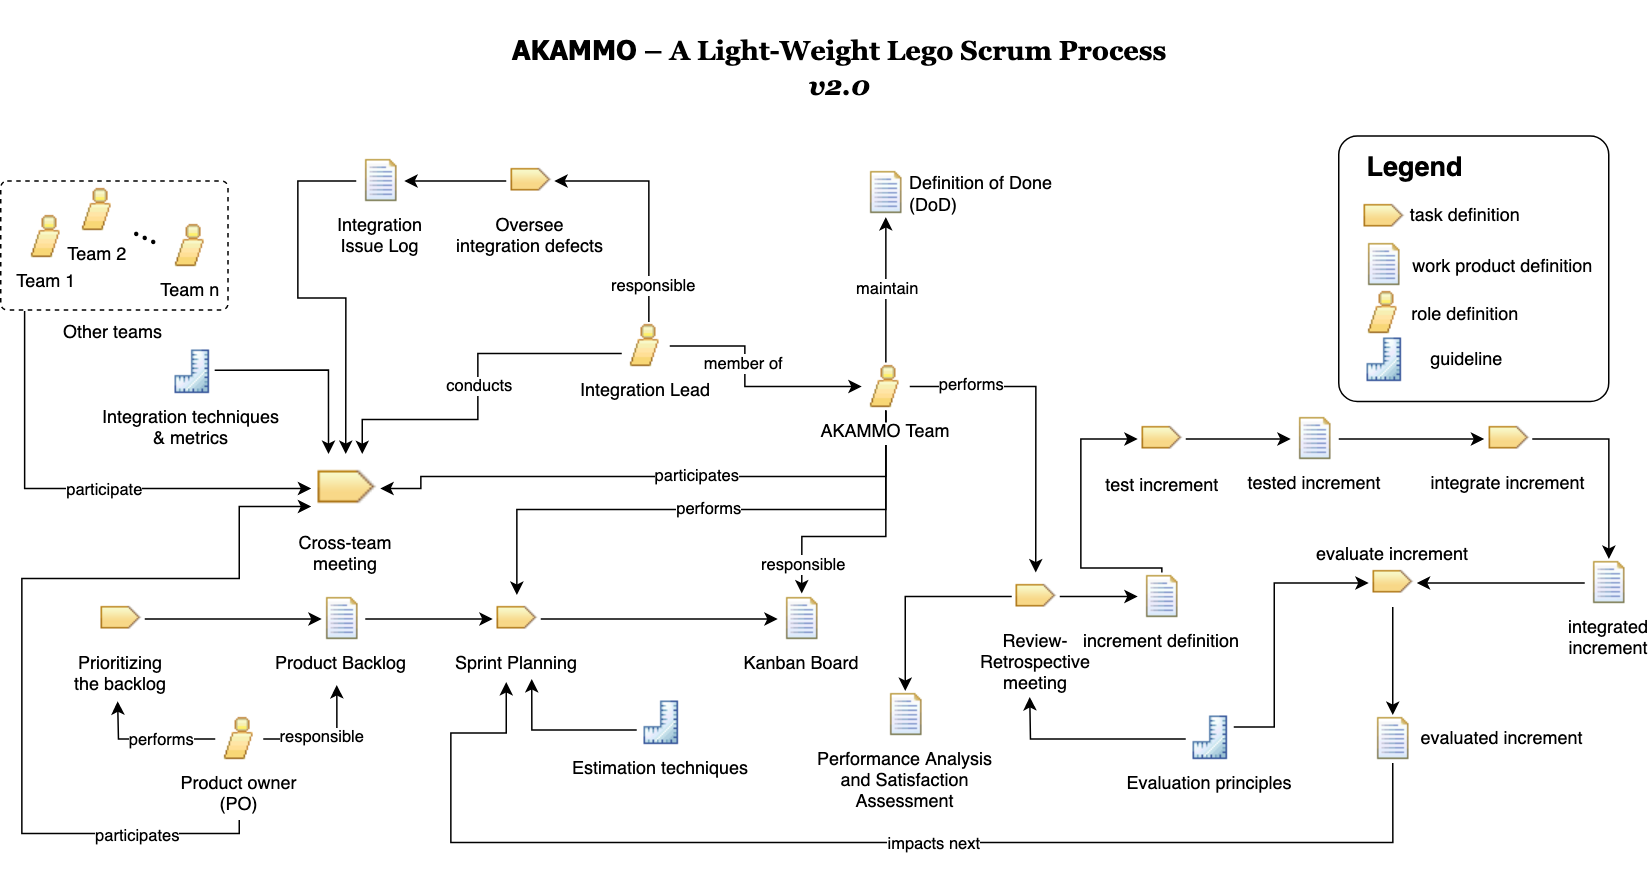
\includegraphics[width=0.9\textwidth]{process-diagram.png}
  \caption{{\fontfamily{qhv}\selectfont AKAMMO} SPEM 2.0 diagram (initial version)}
	\label{fig:process-diagram}
\end{figure*}

\section{Software Process Improvement Techniques}
\label{sec:spi-techniques}

% Provide at least three examples of SPI methods/models/techniques (for an
% overview, see, e.g., \cite{Pettersson2008}). Describe each of them together
% with at least one advantage and one disadvantage.

In our ever-emerging world of software engineering, there is a plethora of SPI
methods, models, and techniques that are available to the practitioners.
Examples of some common SPI models include the Capability Maturity Model
Integration (CMMI), the ISO/IEC 15504 standard, or a more lightweight approach,
the iFLAP model \cite{Pettersson2008}, to name a few. In the following
section, I will briefly describe some of the techniques that are introduced by
iFLAP in relation to the process that was designed for the Lego Scrum workshop.
CMMI and ISO/IEC 15504 are not discussed in this section, since our process is
merely applicable for a small-scale project (with a defined time frame of not
more than four hours), therefore, the aforementioned models may not be suitable
for our endeavor.

\textbf{{\fontfamily{qhv}\selectfont iFLAP}} is an inductive process assessment
framework that largely incorporates the involvement of the practitioners in the
assessment process \cite{Pettersson2008}, \cite{Malvius2009}. Its core
principles are to: (i) construct a feasible selection of roles (and projects),
(ii) gather data points, document them and triangulate the improvement issues,
and (iii) construct an improvement plan based on the analyzed data, identify
dependencies among the improvement issues, and prioritize them; these key
principles [of iFLAP] are adapted from the summary provided by Pettersson et
al. \cite{Pettersson2008}.

A central part of iFLAP is the selection of \textbf{roles} that are to be
involved in the assessment process. This way, once the analysis of the gathered
data is completed, the findings represent viewpoints of a broader spectrum
which is beyond the team's level. Having applied such a technique to our
process, we would, for instance, be able to obtain insights from the PO(s),
team members, the instructor(s), other teams, scrum masters, and so forth. This
would allow us to identify the shortcomings of the process from the perspective
of different actors. As a result, the concern that was discussed, for instance,
in Section~\ref{sec:experiences} about the lack of cross-team communication
would inherently diminish, since the technique induces a need to communicate on
a wider scale. While the technique appears rather straightforward, it does
present several concerns. The selection of the roles is a time-consuming
process and, consequently, might hinder the progress of the project.
Additionally, biases may influence role selection, and thus the assessment
findings may provide inaccurate and unreliable outcomes.

% TODO: check the two sections before working further on the report.
Furthermore, iFLAP suggests to \textbf{gather data} from the selected roles
through the use of interviews and questionnaires. This would allow us to obtain
a more detailed view of the issues that were encountered during the collective
effort. However, similar to the previous technique, the primary limitation of
this technique is the time that is required to gather the data. Interviews, on
a general note, do provide valuable insights into the aspects discussed, albeit
they tend to be lengthy and time-consuming. Questionnaires, on the other hand,
are rather straightforward to conduct, but they do not provide as much detail
as interviews do; furthermore, an analysis of a questionnaire becomes feasible
with some automated tools or scripts (which is not too difficult to implement).
Nevertheless, having applied this technique to our process, we could leverage
the data gathered to enhance the process in the future stages of its maturity;
for instance, we could identify a new strategy on how DoD is to be formulated
and communicated effectively, or how to more accurately assign story points to
the user stories that are to be implemented.

Ultimately, iFLAP further recommends to identify \textbf{dependencies among
improvement issues} as well as \textit{"package"} the improvement issues into
improvement areas \cite{Pettersson2008}, \cite{Malvius2009}. For instance, the
lack of a DoD is an improvement issue and corresponds to an improvement area of
\textit{quality assurance}. The identification of such dependencies allows the
team to tackle the issues in a more efficient manner. Moreover if a certain
dependency is found, then a successful resolution of one issue might result in
a successful resolution of another issue, or, at least, provide an indication
of how to resolve the latter issue. This technique, under general
circumstances, is rather straightforward to implement; however, an extensive
domain knowledge is required to be able to draw dependencies between the
improvement areas, and, in a larger-scale project, this becomes
resource-intensive. Though, in our case, the technique is relevant and feasible
to implement---it must be, however, assumed that the team members have a
sufficient understanding of the domain (i.e., Lego bricks and their usage) and,
as a result, can draw dependencies between the improvement areas.

% Relate each of those methods/models/techniques to the problems you
% encountered and described in Section~\ref{sec:experiences}.
% Explain whether they are applicable to your issues and why.

\section{SPI Proposal for future Scrum Development Efforts}
\label{sec:proposal}
In this section, you should discuss and explain the concrete SPI steps that you suggest to take in order to improve the process you applied during the first Scrum Lego Workshop. First, define at least three goals for an SPI proposal based on what you wrote in Section~\ref{sec:experiences}. Second, define questions and metrics you connect to those goals.
Then, use the tools that were introduced in the course (e.g., GQM or CMMI roadmaps) to define at least two concrete improvement steps per goal. Also, include a plan for how to measure whether your improvement effort was successful. Be careful to reference the corresponding literature when you mention a tool for the first time.

You can use the results of any of the assignments and in-class exercises for this section. While it is okay if members of the same group provide similar answers, each group member has to formulate this section independently.

If you did not attend the Scrum Lego workshop, base your proposal on your analysis in Section~\ref{sec:experiences}. Follow the same guidelines as above for the Scrum Lego workshop. If you go with this option, use the heading ``SPI Proposal for an Industrial Case Study'' for this section.

\section{Implementation of an SPI Initiative}
\label{sec:implementation}
You implemented an SPI initiative in the second workshop.
Give a summary of at least two actual changes that were implemented by your group. These might differ from your original proposal, since not all of your ideas from the proposal might be feasible. Describe at least two effects of those changes and analyze why these effects manifested themselves.
For the selected changes, provide at least one example of concrete measurements that you have made.

This section should contain the overall result for the entire group. Still, each group member has to formulate this section independently.

If you did not attend the Lego workshops, this section may be dedicated to a discussion of challenges in SPI projects. Find at least four relevant references that mention and analyze challenges and compile an overview of what has been observed in the literature. Relate these challenges to empirical studies that have been published and to your personal experience. Identify the SPI techniques that might help to overcome these challenges. Critically discuss the solution approaches from the papers.

\section{Redesign of the Software Process}
\label{sec:redesign}
After reflecting on the SPI experiences, think about how you would design your process for the Lego workshop if you could do it again.
Create a SPEM 2.0 diagram and replace Figure~\ref{fig:placeholderdiagram} with it.
Briefly describe at least the key task definitions, role definitions, and work product definitions that you aim to use, with 1--2 sentences per definition.

This section must be worked on individually.

\section{Bonus Task: Scrum of Scrums}
\label{sec:bonus_task}
This task needs to be solved to get a 5 (pass with distinction).
Note that to get a 5, all other tasks need to be at a level that fulfill the criteria for a 4.
The bonus task cannot be used to pass the exam if you would fail it based on the other tasks.
It cannot be used to improve a 3 (pass) either.

In the workshops, you observed many issues that related to inter-team coordination. One way to address those issues is to have more frequent Scrum of Scrum meetings. Another way to solve them is to have coordination artifacts that create a common understanding between different teams. Find at least three different peer-reviewed sources in the literature that discuss inter-team coordination and/or Scrum of Scrum meetings. Explain at least two challenges that have been reported connected to Scrum of Scrum meetings. Explain and justify whether you would recommend big companies to rely on frequent Scrum of Scrum meetings or whether you think other mechanisms are better for inter-team coordination. 

If you decide to submit the bonus task, you get 1/2 page for it. The new page limit will be 6.5 pages.

\section{Summary and Lessons Learned}
\label{sec:summary}
In the summary section, you should briefly summarize what your report is about and present your main findings/consequences.

This section must be worked on individually.

% This is used to generate the references section. See mybibfile.bib for the bib sources.
\bibliographystyle{IEEEtran}
\bibliography{mybibfile}
\end{document}

